\section{Scalability, Performance and Resource Management}
\label{ch:perf}
\providecommand{\CollN}{50}\providecommand{\CollDel}{92.6}\providecommand{\CollDelMin}{76}\providecommand{\CollDelMax}{100}\providecommand{\CollRecMean}{8.1}\providecommand{\CollRecMax}{10.25}\providecommand{\CollRecN}{50}\providecommand{\CollRecOK}{23}\providecommand{\CollConvMean}{9.6}\providecommand{\CollConvMax}{15.2}

\providecommand{\HopW}{99.2}\providecommand{\HopH}{57.4}\providecommand{\HopWins}{20}\providecommand{\HopRuns}{20}

\providecommand{\SosAdv}{4.4}

\providecommand{\ThrMaxN}{2000}\providecommand{\ThrMaxRate}{4686}\providecommand{\ThrMidRate}{7029}\providecommand{\ThrMaxAck}{1.0}


Every number here is generated from stored measurements by \texttt{docs/report/evidence/}. The \emph{simulator} (real nodes over an in-memory transport with seeded loss on a virtual clock) and \emph{live devices} (real processes, TCP and timers) are never mixed.

\subsection{Scalability Requirements}
The SRS requires 50 nodes, 90\,\% delivery on 40 nodes at 20\,\% loss, convergence within 15\,s and recovery within 10\,s (Section~\ref{sec:kpi}); sizes above five exist only in the simulator.
\subsection{Workload and Load Model}
Each scenario fixes a topology, per-link loss, 5--40\,ms latency, 10--90 messages and a failure script, repeated over seeds so routing modes see identical traffic. Sweeps vary loss 0--50\,\% (21 nodes) and size 10--65 nodes; throughput uses 100--2\,000 sends; the live run sent 30 SOS with 8 relay failures and 4 gateway outages.

\subsection{Resource Utilization}
\textbf{Simulator:} 65 nodes used about 13\,MB of heap (Table~\ref{tab:scale}). \textbf{Live:} about 55\,MB and 0.2--1.0\,\% of a core per idle process (Table~\ref{tab:live}). \textbf{Storage:} one log row per event; at most 500 held messages. \textbf{Network:} transmissions per delivery in Table~\ref{tab:scale}.
\subsection{Concurrent Processing}
A node is single-threaded and cooperative with no locks. On a three-node line with ACKs, \ThrMidRate\ messages per second were delivered at 1\,000 simultaneous sends and \ThrMaxRate\ per second at \ThrMaxN\ (all ACKed within \ThrMaxAck\,s); the concurrency tests (Chapter~\ref{ch:test}) confirm exactly-once delivery.

\subsection{Scheduling and Synchronization Analysis}
Scheduling is by priority, oldest first on ties, at every hop; its metric is the SOS latency advantage under congestion (Section~\ref{sec:perfresults}), since an idle network has nothing to overtake. No synchronisation primitive is needed: shared state lives on the event-loop thread.

\subsection{Performance Measurement}
One Windows~11 laptop, Python~3.10; live runs used five loopback processes with shortened timers. Memory and CPU come from OS counters, live latency from polling every 20\,ms, and simulator metrics from SQL over the node logs.
\subsection{Performance Results}
\label{sec:perfresults}
\textbf{Reliability under loss} (Figure~\ref{fig:results}a, 21-node grid, 8 seeded runs per point). Delivery stays at or above 98\,\% to 20\,\% loss and falls to 61\,\% at 50\,\%; each lost ACK costs a 4\,s timeout, so median latency goes from tens of milliseconds at 0\,\% to seconds at 20--30\,\%.

\textbf{Scenarios.}
\begin{table}[htbp]
\caption[Results of the seven simulator scenarios]{Results of the seven simulator scenarios (weighted routing; delivery ratio shown as mean (min--max) over the runs)}
\label{tab:scenarios}
\footnotesize
\setlength{\tabcolsep}{4pt}
\begin{tabular}{@{}>{\raggedright\arraybackslash}p{0.148\textwidth}>{\raggedleft\arraybackslash}p{0.063\textwidth}>{\raggedleft\arraybackslash}p{0.057\textwidth}>{\raggedleft\arraybackslash}p{0.057\textwidth}>{\raggedleft\arraybackslash}p{0.194\textwidth}>{\raggedleft\arraybackslash}p{0.051\textwidth}>{\raggedleft\arraybackslash}p{0.068\textwidth}>{\raggedleft\arraybackslash}p{0.068\textwidth}>{\raggedleft\arraybackslash}p{0.137\textwidth}@{}}
\toprule
\textbf{Scenario} & \textbf{Nodes} & \textbf{Loss} & \textbf{Runs} & \textbf{Delivery} & \textbf{Hops} & \textbf{Conv. (s)} & \textbf{Recov. (s)} & \textbf{S\&F flushed / queued} \\ \midrule
baseline\_\allowbreak{}10 & 10 & 5\% & 20 & 100.0\,\% (100--100) & 1 & 5.5 & -- & 7/7 \\
collapse\_\allowbreak{}40 & 40 & 20\% & 50 & 92.6\,\% (79--100) & 4 & 9.6 & 8.1 & 2919/3117 \\
no\_\allowbreak{}gateway & 12 & 5\% & 20 & 100.0\,\% (100--100) & 2 & 5.2 & -- & 207/207 \\
high\_\allowbreak{}loss & 20 & 35\% & 20 & 89.3\,\% (74--100) & 2 & 17.7 & -- & 1045/1076 \\
chain\_\allowbreak{}10hop & 11 & 5\% & 20 & 100.0\,\% (100--100) & 9 & 14.4 & -- & 87/90 \\
hopcount\_\allowbreak{}vs\_\allowbreak{}weighted & 5 & 45\% & 20 & 99.2\,\% (90--100) & 2 & 5.2 & -- & -- \\
priority\_\allowbreak{}load & 16 & 0\% & 20 & 100.0\,\% (100--100) & 2 & 7.6 & -- & 1356/1356 \\
\bottomrule
\end{tabular}
\par\smallskip\footnotesize Hops = median hop count of delivered messages. Conv. = mean seconds until every node's graph contains every node. Recov. = mean seconds from relay death until the sender has a route avoiding it. S\&F counts are event counts summed over all runs: a message re-queued after a failed retry is counted each time, and messages still held when a run ends are not flushed.
\end{table}

The 40-node collapse scenario (20\,\% loss, a relay on the active path killed at $t=10$\,s, the gateway killed at 25\,s and revived at 60\,s) delivered \CollDel\,\% on average over \CollN\ seeded runs (worst \CollDelMin\,\%, best \CollDelMax\,\%). At 35\,\% loss (outside the specified condition) delivery was 89.1\,\%.
\begin{figure}[!tb]
\centering
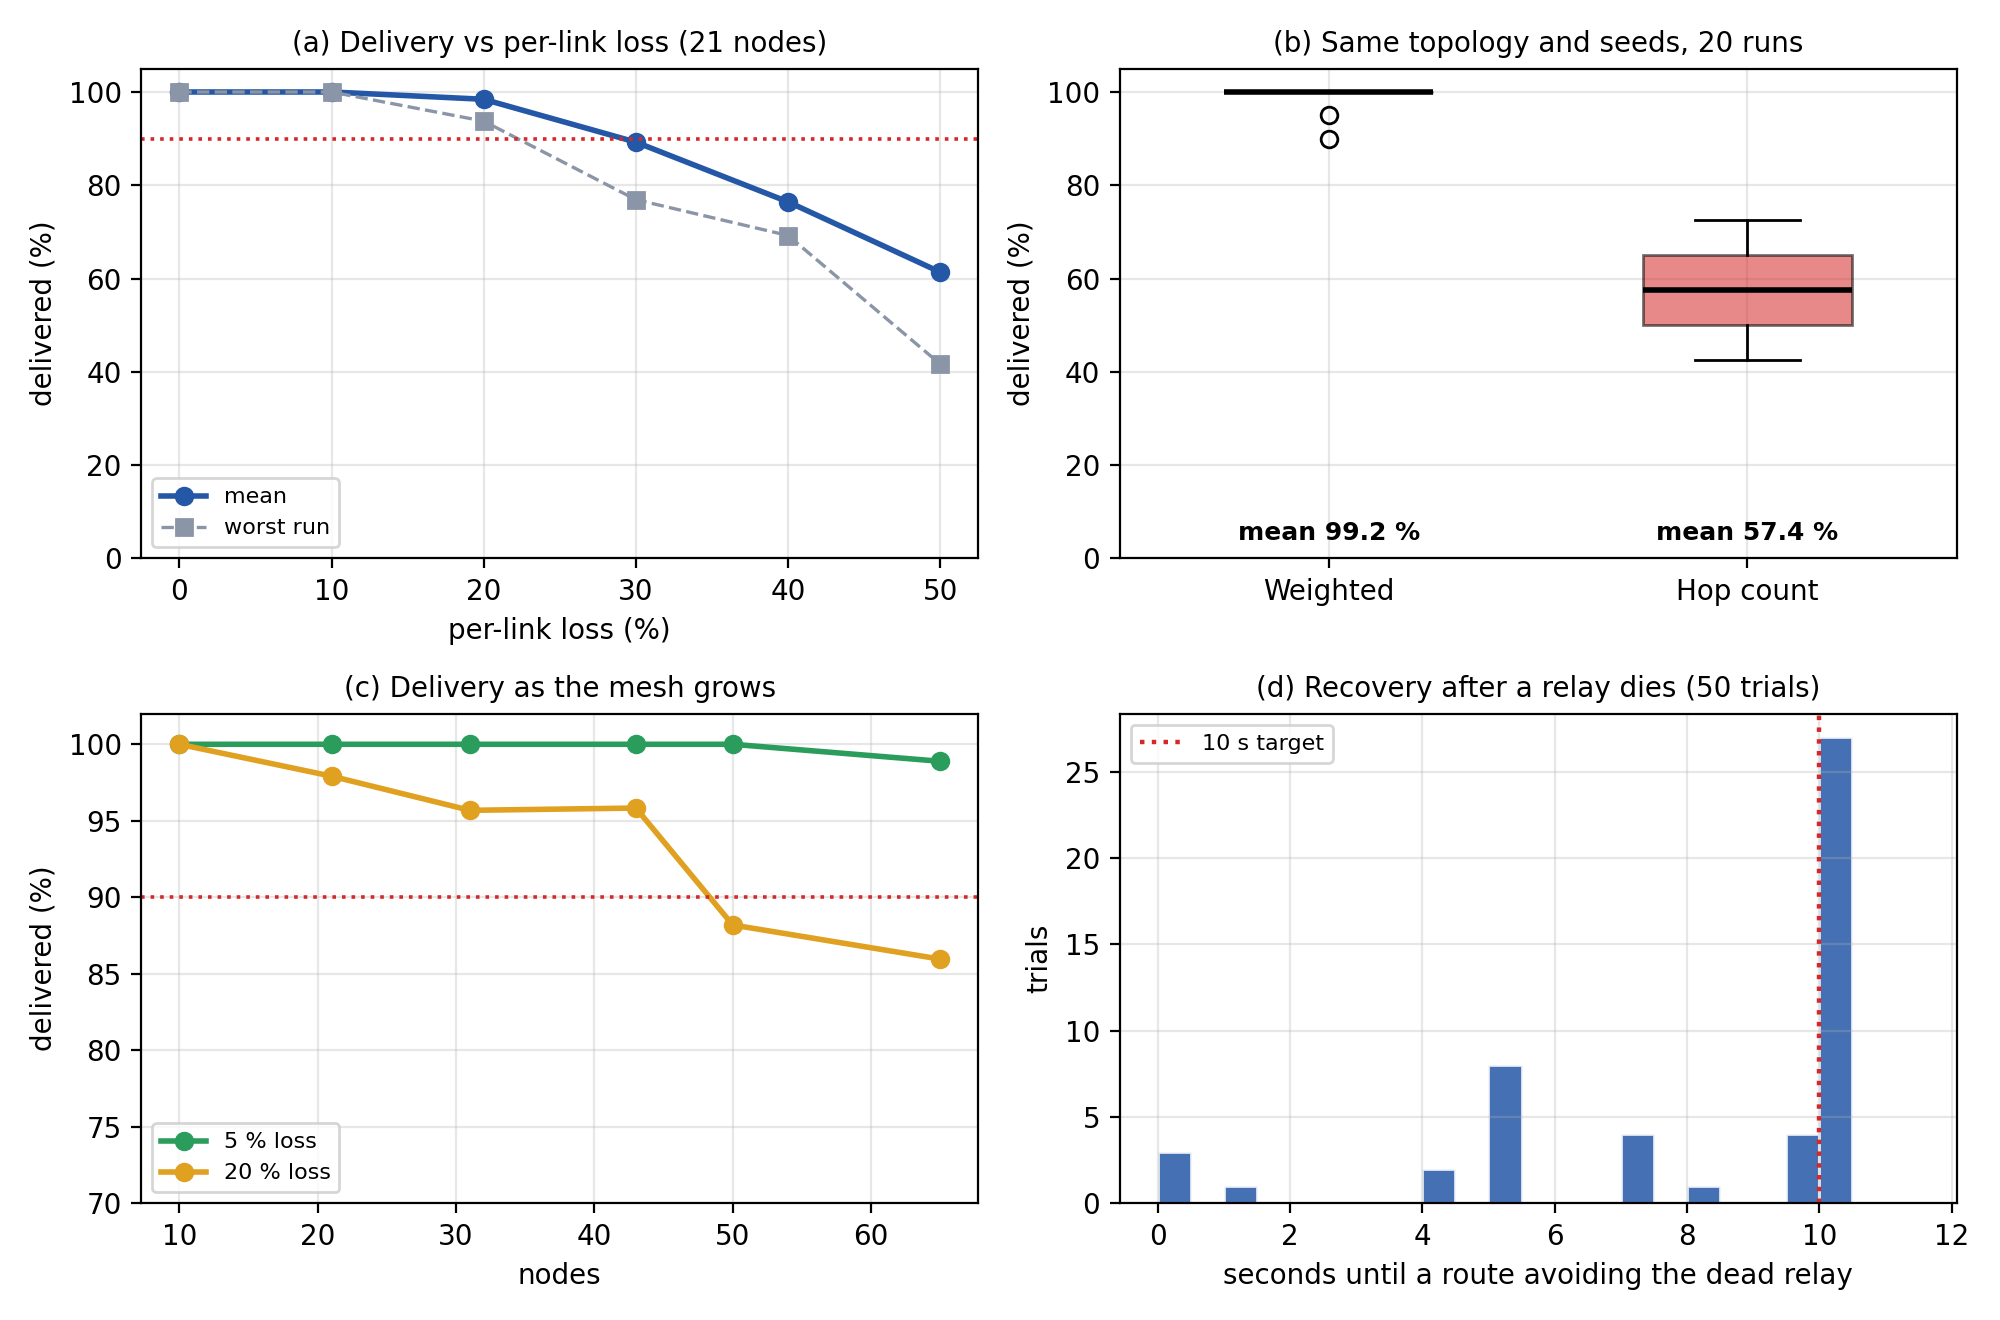
\includegraphics[width=0.86\textwidth]{figures/fig_results.png}
\caption[Delivery, routing comparison, scale and recovery results]{(a) Delivery against per-link loss. (b) Weighted versus hop-count routing on identical seeds. (c) Delivery as the mesh grows. (d) Recovery time after a relay death, 50 trials.}
\label{fig:results}
\end{figure}
\textbf{Weighted versus hop-count routing (Figure~\ref{fig:results}b).} A 2-hop shortcut crosses a link with 45\,\% loss while a 3-hop path is clean, and messages are best-effort, so a poor route shows directly as loss. Weighted routing delivered \HopW\,\% and hop count \HopH\,\%, weighted winning on \HopWins\ of \HopRuns\ identical seeds. The topology is \emph{designed} to expose hop count, so it shows that the cost avoids a lossy shortcut, not that every mesh has this gap.

\textbf{Priority under load.} The congested scenario (16 nodes, 90 messages to the same destination, 15\,\% SOS) gives an SOS a median latency \SosAdv$\times$ lower than routine traffic. Only here do both take the same trip, so the comparison is fair.

\textbf{Scalability.}
\begin{table}[htbp]
\caption[Scalability, 10 to 65 simulated nodes]{Scalability, 10 to 65 simulated nodes (10 runs per size and loss rate)}
\label{tab:scale}
\footnotesize
\setlength{\tabcolsep}{4pt}
\begin{tabular}{@{}>{\raggedleft\arraybackslash}p{0.077\textwidth}>{\raggedleft\arraybackslash}p{0.077\textwidth}>{\raggedleft\arraybackslash}p{0.100\textwidth}>{\raggedleft\arraybackslash}p{0.100\textwidth}>{\raggedleft\arraybackslash}p{0.100\textwidth}>{\raggedleft\arraybackslash}p{0.100\textwidth}>{\raggedleft\arraybackslash}p{0.115\textwidth}>{\raggedleft\arraybackslash}p{0.084\textwidth}>{\raggedleft\arraybackslash}p{0.092\textwidth}@{}}
\toprule
\textbf{Nodes} & \textbf{Links} & \textbf{Delivery at 5\% loss} & \textbf{Delivery at 20\% loss} & \textbf{Tx per delivered (5\%)} & \textbf{Tx per delivered (20\%)} & \textbf{Conv. max at 20\% (s)} & \textbf{CPU (s, 5\%)} & \textbf{Heap (MB, 5\%)} \\ \midrule
10 & 13 & 100.0\,\% & 100.0\,\% & 5.0 & 8.9 & 15.2 & 3 & 0.7 \\
21 & 32 & 100.0\,\% & 98.8\,\% & 7.4 & 16.1 & 15.2 & 13 & 1.7 \\
31 & 50 & 100.0\,\% & 96.2\,\% & 10.6 & 26.5 & 15.2 & 43 & 3.0 \\
43 & 72 & 100.0\,\% & 96.2\,\% & 12.2 & 24.8 & 20.2 & 91 & 5.3 \\
50 & 85 & 100.0\,\% & 92.9\,\% & 14.2 & 31.9 & 15.2 & 110 & 6.5 \\
65 & 113 & 98.0\,\% & 83.1\,\% & 20.6 & 39.4 & 15.2 & 188 & 9.8 \\
\bottomrule
\end{tabular}
\par\smallskip\footnotesize Nodes and links include the gateway and rescue post added to the grid. Tx = hop-by-hop data transmissions. CPU and heap are for the whole simulated mesh in one process on a virtual clock, not the cost of one real device.
\end{table}

At 5\,\% loss delivery is 100\,\% to 50 nodes and 98.0\,\% at 65; at 20\,\% loss it is 92.9\,\% at 50 and 83.1\,\% at 65. Transmissions per delivery grow about linearly with size, not quadratically as with flooding.

\textbf{Recovery and convergence} follow the timers (Figure~\ref{fig:results}d): convergence comes in multiples of the 5\,s gossip interval, and recovery took under 10\,s in 24 of 50 trials and 10.2--10.25\,s in the rest, bounded by the 10\,s heartbeat timeout.

\textbf{Live devices.} Table~\ref{tab:live} gives five real processes over real TCP.
\begin{table}[H]
\caption{Live devices: 5 operating-system processes, real TCP sockets, real timers, on one laptop (loopback)}
\label{tab:live}
\footnotesize
\setlength{\tabcolsep}{4pt}
\begin{tabular}{@{}>{\raggedright\arraybackslash}p{0.482\textwidth}>{\raggedright\arraybackslash}p{0.482\textwidth}@{}}
\toprule
\textbf{Measurement} & \textbf{Result} \\ \midrule
Process start \textrightarrow{} every device knows every device & 3.8 s \\
SOS arrives at the rescue device (30/30 delivered) & median 47 ms, 95th pct 102 ms, max 281 ms \\
ACK back at the sender & median 63 ms, 95th pct 149 ms \\
Relay switched off \textrightarrow{} sender re-routes (8 trials) & median 4.0 s, max 4.5 s; every later SOS delivered \\
Gateway down, 5 SOS held; gateway back (4 trials) & 100\% flushed, median 4.5 s, max 6.1 s \\
Device API response (200 requests) & median 16 ms, 95th pct 31 ms \\
Per-process memory and CPU, idle & 53--54 MB; 0.4--1.9\% of one core \\
Per-process CPU while sending SOS (includes the harness polling every 20 ms) & up to 19\% of one core \\
\bottomrule
\end{tabular}
\par\smallskip\footnotesize Timer settings: HELLO 1 s, neighbour timeout 4 s, link-state 2 s, ACK timeout 3 s. Latency is measured by polling each device's own API every 20 ms (up to 20 ms of error). Wireless delay and loss are not included.
\end{table}


\subsection{Bottleneck Identification}
The 10\,s heartbeat timeout (which bounds recovery), the 4\,s ACK timeout under loss, the 5\,s link-state interval, one SQLite commit per event and whole-cache route invalidation.
\subsection{Optimization and Improvement}
No optimisation followed these measurements, so there is no before-and-after comparison; the data point to a shorter, adaptive neighbour timeout, an immediate link-state report on change, an adaptive ACK timeout and per-destination invalidation.
\subsection{Cloud Deployment and Resource Utilization}
Not applicable: there is no server and no cloud deployment.
\subsection{Scalability Limitations}
Tested to 65 simulated nodes and 5 live devices; larger meshes, wireless interference and mobility were not tested.
